%!TEX root = Master.tex

%----------------------------------------------------------------------------------------
%	PACKAGES AND OTHER DOCUMENT CONFIGURATIONS
%----------------------------------------------------------------------------------------

\documentclass{report}

\usepackage{graphicx}
\usepackage{hyperref}
\usepackage{fixme} \fxsetup{status=draft}
\usepackage{amsmath,amsfonts,amssymb}
\usepackage{geometry}

\setlength{\parindent}{0cm}
%----------------------------------------------------------------------------------------
%	TITLE SECTION
%----------------------------------------------------------------------------------------

\title{
	\textbf{AI in Robotics}
}

\author{
	Line Aggerbo, Rasmus S. Reimer \& Kasper D. Saaby\\
	Aarhus University, Department of Engineering \\
}
\date{\today}

%----------------------------------------------------------------------------------------

\begin{document}

\maketitle

%----------------------------------------------------------------------------------------
%	ABSTRACT
%----------------------------------------------------------------------------------------

\begin{abstract}
The Content of this paper seeks to present the knowledge gained throughout the non-linear signal processing and pattern recognition course from Aarhus University, department of engineering. The paper is split into multiple sections explaining the data used in the paper, the methods used to process the data and the methods used for categorising the data. The results are presented along with a discussion of the results.
\fxnote{Rewrite the abstract}
\end{abstract}


%----------------------------------------------------------------------------------------
%	ARTICLE CONTENTS
%----------------------------------------------------------------------------------------
\chapter{Theory}
%!TEX root = ..\Master.tex

\section{Dimensionality Reduction}
\fxnote{Remove this section from the report.}

%e.g. finding projection vectors, choosing number of components, applications.\\
%motivation:
%data compression
%speed up learning algorithm
When working with large amounts of data in higher dimensions you often need a lot of computing power. Dimensionality reduction is mostly used in order to speed up the learning algorithm. This section contains an explanation of two widely used dimensionality reduction methods, Principal component analysis (PCA) and Fisher Discriminant method (Fisher).


\subsection{PCA}

PCA is used for reducing the number of dimensions of a feature space.
It works by projecting the data in the feature space, down to a fewer dimensional feature space by minimizing the squared projection error.
The reduced feature space does not nessecarily share the same features, but new features are found which best retains the variance in the data.

PCA should mainly be used for compressing the data to save memory or reducing running time of learning algorithm.
By reducing the amount of features most machine learning algorithms runs faster.
PCA can also be used to prevent overfitting, but it is usually better to use regularization. \\

Figure \ref{fig:pca} shows a 3 dimensional feature space where all the data, within a small margin, lies in a 2 dimensional plane.
PCA is used to find two vectors $u^{(1)}$ and $u^{(2)}$ which spans this 2D plane.

\begin{figure}
\centering
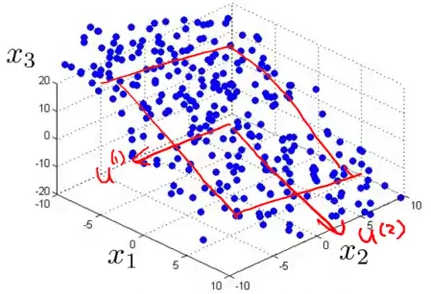
\includegraphics{images/pca}
\caption{3D to 2D PCA illustration}
\label{fig:pca}
\end{figure}

The plane is the 2 dimensions, in which the most variance is obtained in the data. Preprocessing of the data should be done before doing PCA. Given the training set:
\begin{equation}
x = 
\begin{bmatrix}
x_1 & x_2 & \dots & x_m
\end{bmatrix}
\end{equation}

Ensure that every feature has zero mean by doing mean normalization:
\begin{equation}
\mu_j = \frac{1}{m} \sum^m_{i=1} x_j^{(i)}
\end{equation}
\begin{equation}
x_j = x_j - \mu_j
\end{equation}

After preprocessing the data, we can do PCA on it. We start by computing the covariance matrix $\Sigma$:

\begin{equation}
\Sigma = \frac{1}{m} \sum^n_{i=1} x^{(i)} {x^{(i)}}^T
\end{equation}

The covariance matrix describes how the different features relates. When doing feature reduction we want to remove features which has high correlation with other features.
An example could be a feature which describes a length in cm and another feature describing the same length in inches.
These features will have very high correlation and one of them can be removed from the feature space without loosing much information. \\

Then we compute the eigenvectors of covariance matrix:
\begin{equation}
U = \begin{bmatrix}
   u^{(1)} & u^{(2)} & \dots & u^{(n)}
 \end{bmatrix}
\in \mathbb{R}^{n \times n}
\end{equation}

The eigenvectors will lay in the directions of most variance in the data. This is what is shown on Figure \ref{fig:pca}.
The longer the eigenvector, the more variance it describes.
Therefore we want to keep the longest eigenvectors and remove the shortest eigenvectors. The eigenvectors are ordered by length in the matrix $U$.  We select the first $k$ eigenvectors to get the reduced set of eigenvectors:

\begin{equation}
U_{reduce} = \begin{bmatrix}
   u^{(1)} & u^{(2)} & \dots & u^{(k)}
 \end{bmatrix}
\end{equation}

We can now calculate the new feature vectors:
\begin{equation}
z = U_{reduce}^Tx
\end{equation}

We have now reduced the feature space to a $k$ dimensional feature space.
Say we want to retain at least $95\%$ of the variance in the data.
We do this by picking the smallest value of $k$ so that:
\begin{equation}
\frac{\displaystyle\sum^{k}_{i=1} S_{ii}}{\displaystyle\sum^{n}_{i=1} S_{ii}} \geq 0.95
\end{equation}

The matrix $S$ is found by doing singular value decomposition (SVD). The matrix $S$ has the form:
\begin{equation}
S =  
\begin{bmatrix}
S_{11} & 0 & 0 & 0 & 0 \\
0 & S_{22} & 0 & 0 & 0 \\
0 & 0 & S_{33} & 0 & 0 \\
0 & 0 & 0 & \dots & 0 \\
0 & 0 & 0 & 0 & S_{nn} \\
\end{bmatrix}
\end{equation}

In our project we use PCA to reduce our feature space from 64 dimensions down to 40 dimensions.
We do this to increase the speed of our learning algorithms while still retaining almost all of our data ($\geq 99.99\%$) as seen on Figure \ref{fig:pca-on-our-data}.

\begin{figure}
\centering
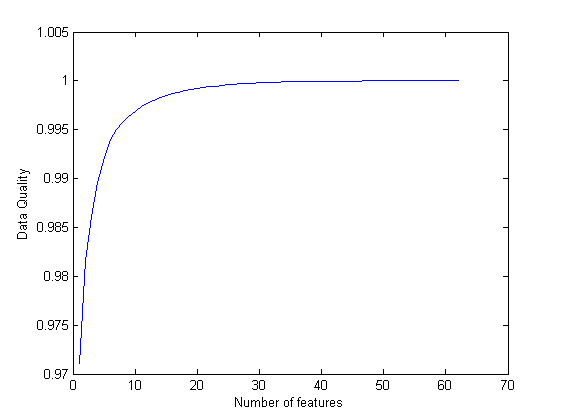
\includegraphics[scale = 0.8]{images/pca-on-our-data}
\caption{ Retained variance per dimension}
\label{fig:pca-on-our-data}
\end{figure}

\subsection{Fisher}
Fisher's linear discriminant is another look on dimensionality reduction. Instead of maximizing the variance of the data, we use the information we have on the classes to separate them as much as possible. We use equation \ref{fisher1} and place a threshold on y such that class 1: $y\geqslant -\omega_0$ and class 2 is everything else. This is also said as projecting data down to one dimension.
\begin{equation}
\label{fisher1}
y = \textbf{w}^T\textbf{x}
\end{equation}
This leads to a considerable loss in information and may cause overlapping in data that did not overlap in multidimensional space as can be see on figure \ref{fig:fisher} from the book Pattern Recognition and Machine Learning by Christopher M. Bishop\cite{bishop2006pattern}. The left Image is  the original space while the right image is in the projected space.\\
\begin{figure}
\centering
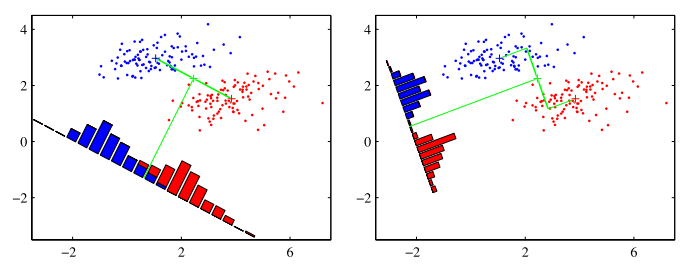
\includegraphics[width=1\textwidth]{images/fisher}
\caption{Picture from the Pattern Recognition and Machine Learning Book by Christopher M. Bishop}
\label{fig:fisher}
\end{figure}
By adjusting the weight vector \textbf{w} a solution can be found that minimises overlapping by maximising the distance between classes. Given two classes we have:
\begin{equation}
m_1 = \frac{1}{N_1} \sum_{n=C_1} X_n,       m_2 = \frac{1}{N_2} \sum_{n=C_2} X_n
\end{equation}
With \textbf{m} being the mean of the class and \texttt{N} being the amount of points in the class. The goal is to maximise the difference $m_2 - m_1$ and this is done by maximising the difference of the projected data as well:
\begin{equation}
m_2 - m_1 = \textbf{w}^{T} \times ( \textbf{m}_2 - \textbf{m}_1 )
\end{equation}
We add the constraint that $\sum_i \omega^2_i  = 1$ in order to avoid large expressions when dealing with the projected data. When solving this we see that there might be an issue with considerable overlap in the projected space.\\
The fisher method seeks to minimise the class overlap by reducing in class variance. Within-class variance is given by:
\begin{equation}
s^2_k = \sum_{n=C_1} (y_n - m_k)^2
\end{equation}
where $y_n = \textbf{w}^T\textbf{x}_n$ and $m_k$ is the difference mentioned earlier. The fisher criterion is given by:
\begin{equation}
J(\textbf{w})=\frac{(m_2 - m_1)^2}{s^2_1+s^2_2}
\end{equation}
This can also be written as:
\begin{equation}
J(\textbf{w})=\frac{\textbf{w}^T\textbf{S}_B\textbf{w}}{\textbf{w}^T\textbf{S}_W\textbf{w}}
\end{equation}
Where $\textbf{S}_B = (\textbf{m}_2 - \textbf{m}_1)(\textbf{m}_2 - \textbf{m}_1)^T$ is the between-class covariance matrix and $\textbf{S}_W = \sum_{n\in C_1}(\textbf{x}_n - \textbf{m}_1)(\textbf{x}_n - \textbf{m}_1)^T + \sum_{n\in C_2}(\textbf{x}_n - \textbf{m}_2)(\textbf{x}_n - \textbf{m}_2)^T $ is the within-class covariance matrix.
Differentiating and removing the scaling factors we get:
\begin{equation}
\textbf{w} \propto \textbf{S}^-1_W ( \textbf{m}_2 - \textbf{m}_1 )
\end{equation}
This is know as Fisher's linear discriminant. This holds for 2 classes but in this project there is 3 classes. A general term for Fisher's discriminant for more than two classes must be considered.\\
Given $\textbf{y} = \textbf{W}^T\textbf{x}$ where \textbf{W} is the weight vectors $\textbf{w}_k$. The within-class covariance for K classes is given by: 
\begin{equation}
\textbf{S}_W = \sum^K_{n=1} \sum_{n=C_k} (\textbf{x}_n - \textbf{m}_k)(\textbf{x}_n - \textbf{m}_k)^T 
\end{equation}
With $\textbf{m}_k = \frac{1}{N_k}\sum_{n=C_k} \textbf{x}_n$, $N_k$ is the number of patterns in class k. The total covariance matrix given by Duda and Hart(1973) is used to find the between-class covariance matrix.
\begin{equation}
\textbf{S}_T = \sum^N_{n=C_k}(\textbf{x}_n - \textbf{m})(\textbf{x}_n - \textbf{m})^T 
\end{equation}
where \textbf{m} is the mean of the total data set. The between class covariance matrix can be found by using $\textbf{S}_T = \textbf{S}_W + \textbf{S}_B$.
\begin{equation}
\textbf{S}_B = \sum^N_{n=C_k} N_k(\textbf{m}_k - \textbf{m})(\textbf{m}_k - \textbf{m})^T 
\end{equation}
Defining these matrices in the projected space we get:
\begin{equation}
\textbf{s}_W = \sum^K_{n=1} 
\sum_{n=C_k} (\textbf{y}_n - 
\boldsymbol{\mu}_k)
(\textbf{y}_n - 
\boldsymbol{\mu}_k)^T 
\end{equation}
\begin{equation}
\textbf{s}_B = \sum^N_{n=C_k} N_k(\boldsymbol{\mu}_k - \boldsymbol{\mu})(\boldsymbol{\mu}_k - \boldsymbol{\mu})^T 
\end{equation}
where $\boldsymbol{\mu}_k = \frac{1}{N_k}\sum_{n=C_k}\textbf{y}_n$ 
and $\boldsymbol{\mu} = \frac{1}{N_k}\sum^K_{k=1}N_k \boldsymbol{\mu}_k$.\\
The cost function is then defined as:
\begin{equation}
J(\textbf{W}) =  Tr\{\textbf{s}^{-1}_W\textbf{s}_B\}
\end{equation}
The means and covariances are estimated from the training set. The resulting dimensions is K - 1  where K is the number of classes. In this project the dimensions of the fisher linear discriminant is $3 - 1 = 2$. Analysing these projected features does not provide distinct classes in this project. An examples of this is found in the linear classifier section when plotting 2 dimensional features.

%------------------------------------------------
%!TEX root = ../Master.tex

\section{Localization} % (fold)
\label{sec:localization}

Localization is used when a given robot has no idea of where it is located. The localization tasks consists of two main tasks; sensing and moving. These two tasks are performed alternately as illustrated in \autoref{fig:main tasks}. The robot might have an initial belief of where it is located and in that case this belief is taken into account together with the sense task at first. For the robot to use localization it must be in possession of a map of the environment. The robot uses the map to compare it's belief of it's localization with the results of the sensing and the map.\\

\begin{figure}[H]
\centering
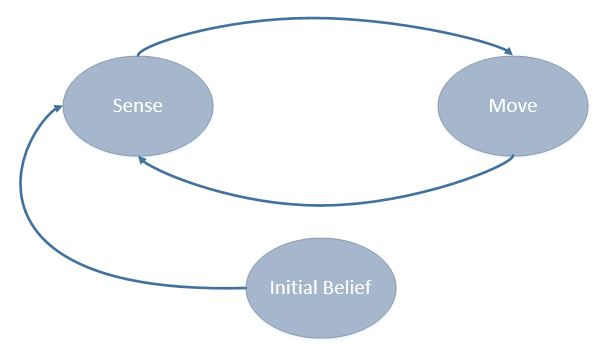
\includegraphics[scale=0.45]{images/SenseMoveInitialBelief}
\caption{Main tasks of localization}
\label{fig:main tasks}
\end{figure}

The first of the two tasks for the robot is to sense. This in done by using the sensors which are built in to the robot. As an example the robot could measure the distance to all walls in the environment or the color of the floor. These measurements should lead to a better belief of where the robot is located. Every time the robot senses it gains information of where it is located. The second task for the robot is to move. The robot needs to move in order to be able to get new information from the sensing task. When the robot moves it looses information of where it is located. This is due to inaccuracy of the robots speed and orientation. This will be illustrated in a robot example later on in this section.\\

The algorithm to implement the two tasks is called the Markov Localization algorithm and is illustrated in Algorithm \ref{alg:ml_def1}. The algorithm is based on the Bayes filter algorithm and calculates the new belief based on the old belief $bel(x_{(t-1)})$, the motion $u_t$, the measurements $z_t$ and the map.

\begin{center}
\begin{minipage}{.65\linewidth}
\alglanguage{pseudocode}
\begin{algorithm}[H]
\caption{Markov Localization}
\label{alg:ml_def1}
\begin{algorithmic}[1]
\Procedure{MarkovLocalization}{$bel(x_{t-1}),u_{t},z_{t},m$}
  \ForAll{$x_{t}$}
    \State $\overline{bel}(x_{t}) = \int{p(x_{t}|u_{t},x_{t-1},m)bel(x_{t-1})dx}$
    \State $bel(x_{t}) = \eta\;p(z_{t}|x_{t},m)\overline{bel}(x_{t})$
  \EndFor
  \State \textbf{return} $bel(x_{t})$
\EndProcedure
\end{algorithmic}
\end{algorithm}
\end{minipage}
\end{center}

The first step in the algorithm is line 3 in Algorithm \ref{alg:ml_def1}. In this line the algorithm calculates the sum of the product of two distributions. The two distributions are the prior belief of the robot being at the position $x_{t-1}$ and the probability that the motion $u_t$ moved the robot from the position $x_{t-1}$ to the new position $x_t$ according to the map. This step in the algorithm is referred to as the motion update. \\

The second step is line 4 in Algorithm \ref{alg:ml_def1}. This step looks at the probability that the measurement $z_t$ may have been observed at the the location $x_t$ according to the map. This is multiplied by the belief of $x_t$. This product is normalized by the normalization constant $\eta$ so it will integrate to 1. This step is referred to as the measurement update.\\

The algorithm needs a prior belief to calculate the new belief. If no initial belief is known the algorithm should use a uniform distribution as the prior belief.

\subsection{Robot Example} % (fold)
\label{sub:robot_example}

This is an example of the localization process where a robot has to localize itself. In \autoref{fig:initialBelief} the scenario is illustrated. The robot is in an environment with three doors. The robot has no idea of where it is located and the initial belief $bel(x)$ is therefore a uniform distribution.

\begin{figure}[H]
\centering
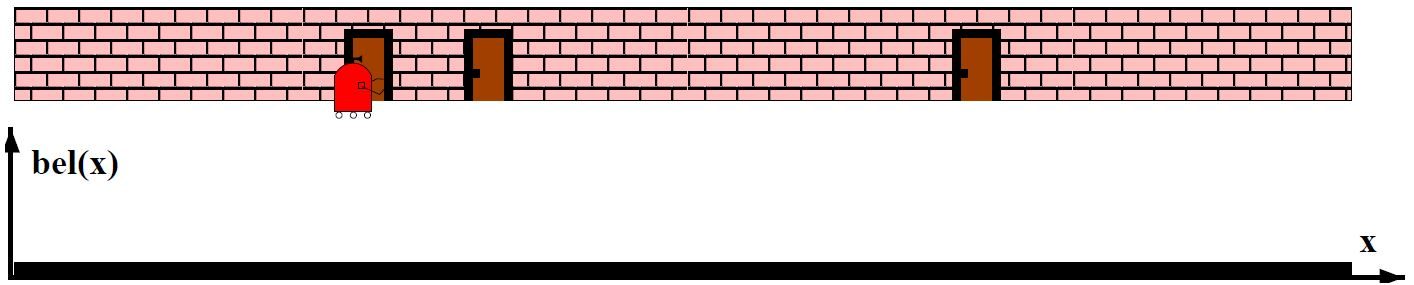
\includegraphics[scale=0.36]{images/MarkovLocalizationA}
\caption{The initial belief of the robot's location}
\label{fig:initialBelief}
\end{figure}

As the robot starts localizing itself it performs a sensing task. The measurement indicates that the robot is located next to a door. This measurement should only be obtained at three different locations in this environment. The probability of obtaining this measurement when located at those three locations, $p(z|x)$, therefore increases as illustrated in \autoref{fig:afterSenseBelief}. The new belief is calculated as the product of the prior belief and this probability.

\begin{figure}[H]
\centering
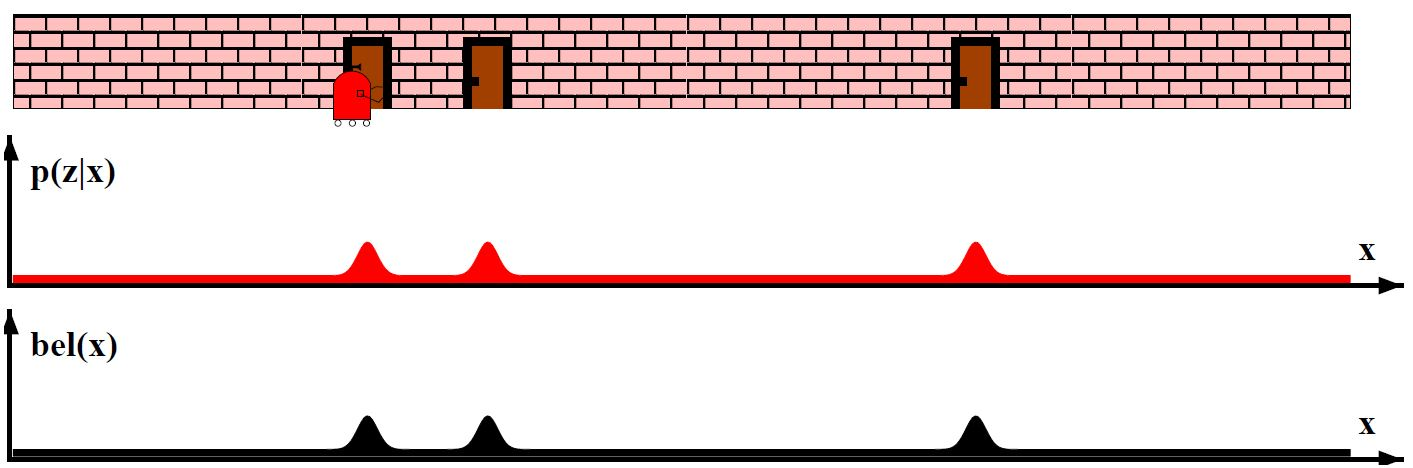
\includegraphics[scale=0.36]{images/MarkovLocalizationB}
\caption{The belief of the robot's location after sensing}
\label{fig:afterSenseBelief}
\end{figure}

The next task for the robot is the moving task. The robot moves a little to the right as illustrated in \autoref{fig:afterMoveBelief}. The belief is now a little less sure of the three most possible locations. This is due to inaccuracy as described earlier in this section.

\begin{figure}[H]
\centering
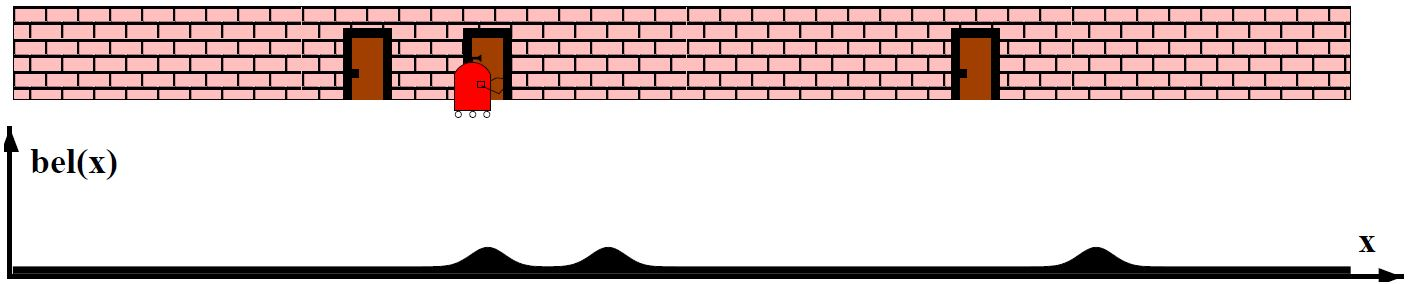
\includegraphics[scale=0.36]{images/MarkovLocalizationC}
\caption{The belief of the robot's location after moving}
\label{fig:afterMoveBelief}
\end{figure}

The robot performs a new sense task and the measurement indicated that the robot is located at a door which leads to a probability similar to the one obtained after the first sensing task. This time, as last time, it is multiplied by the prior belief. This results in a new belief with only one dominant location as illustrated in \autoref{fig:afterSecondSenseBelief}. 

\begin{figure}[H]
\centering
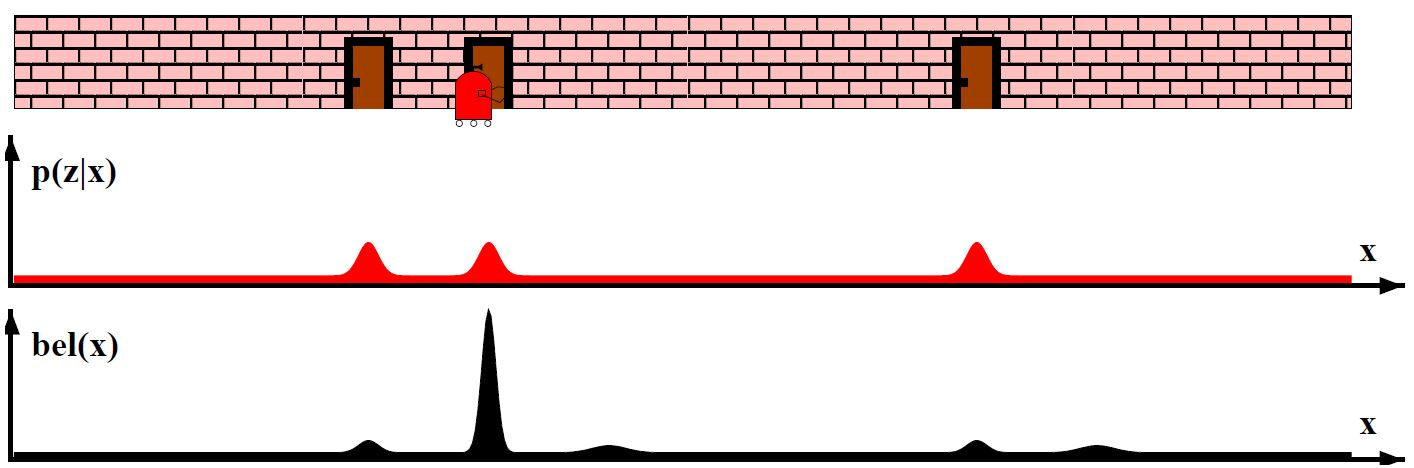
\includegraphics[scale=0.36]{images/MarkovLocalizationD}
\caption{The belief of the robot's location after second sensing}
\label{fig:afterSecondSenseBelief}
\end{figure}

Even though the robot moves the one location is still dominant as illustrated in \autoref{fig:finalBelief}. Hence only one location is dominant and the robot has now localized itself.

\begin{figure}[H]
\centering
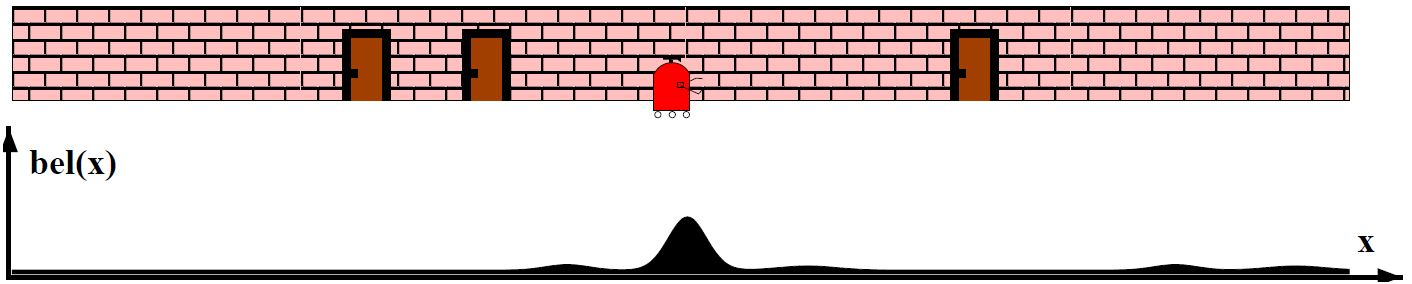
\includegraphics[scale=0.36]{images/MarkovLocalizationE}
\caption{The robot localizes itself}
\label{fig:finalBelief}
\end{figure}

% subsection robot_example (end)

% section localization (end)

%!TEX root = ../Master.tex

\section{Kalman filters}

The Kalman filter (KF) is a technique for filtering and prediction in linear systems. In the context of robotics the filter can be used to locate the robot and make predictions as to where the robot will reside in the next time-step.\\

The technique makes it possible to do data fusion, which is the process of combining observations from a number of different sensors to provide a robust and complete description of the environment. Robots could e.g. use radar, lidar, GPS, compass, camera, etc. for location and combining these sensor informations would result in are more complete overview of the robot and its environment.\\

The KF consists of a basic cycle which includes making predictions and updating these predictions with actual measurement data. The filter represents it's beliefs about state of the system as a Gaussian distribution which is characterized by two parameters: the mean value $\mu$ and the variance $\sigma^2$. Another important property of the KF and Gaussians is that they are unimodel. This means that they posses a single maximum as opposed to e.g. Particle Filters and Monte Carlo Localization which are multimodal.\\

The formal definition of the KF algorithm is given in Algorithm \ref{alg:kf_def1}. Notice that the variance is now represented by $\Sigma_{t}$ which in higher dimensional spaces denotes an covariance matrix.

\begin{center}
\begin{minipage}{.65\linewidth}
\alglanguage{pseudocode}
\begin{algorithm}[H]
\caption{Kalman Filter}
\label{alg:kf_def1}
\begin{algorithmic}[1]
\Procedure{KalmanFilter}{$\mu_{t-1},\Sigma_{t-1},u_{t},z_{t}$}
  \State $\bar\mu_{t} = A_{t}\mu_{t-1} + B_{t}u_{t}$%\Comment{This is a comment}
  \State $\bar\Sigma_{t} = A_{t}\Sigma_{t-1}A_{t}^T + R_{t}$
  \State $K_{t} = \bar\Sigma_{t}C_{t}^T(C_{t}\bar{\Sigma}_{t}C_{t}^T+Q_{t})^{-1}$
  \State $\mu_{t} = \bar\mu_{t} + K_{t}(z_{t} - C_{t}\bar\mu_{t})$
  \State $\Sigma_{t} = (I - K_{t}C_{t})\bar\Sigma_{t}$
  \State \textbf{return} $\mu_{t}, \Sigma_{t}$
\EndProcedure
\end{algorithmic}
\end{algorithm}
\end{minipage}
\end{center}

The algorithm takes four parameters: The previous mean value and variance of the system $\mu_{t-1}$ and $\Sigma_{t-1}$, respectively, the new control-input $u_{t}$ and measurement data $z_{t}$. In line 2 the previous mean value and control-input are mapped into the new mean value $\bar{\mu_{t}}$ which is a prediction of the system state. In line 3 the variance is propagated together with the measurement noise $R_{t}$. In line 4 the Kalman gain is calculated, which is used as a weight factor in line 5 to determine the degree to which we believe in the measurement as opposed to the prediction. Lastly the variance is updated in line 6.\\

The mean value of the system could be a position, velocity or a heading. The transition matrix $A_{t}$ applies the effects of $\mu_{t-1}$ on $\mu_{t}$, and the transition matrix $B_{t}$ applies the effects of control-input $u_{t}$ on $\mu_{t}$. The factors $R_{t}$ and $Q_{t}$ models the motion noise and measurement noise, respectively. In higher dimensional spaces these will be covariance matrices.\\

As mentioned, the KF represents its beliefs about the system, predictions and measurements, as Gaussians. An important property of the KF is that combining the predictions and the measurements increases the certainty about the system state. Gaussians has the characteristic that multiplying two Gaussians produces a new Gaussian with a variance that is smaller than the variance of both of the original Gaussians, and therefore this new Gaussian will have a larger peak than the original Gaussians. The mean value of the new Gaussian will lie between the two mean values of the two original Gaussians. \\

The measurement update consists of the multiplication of the prediction and the measurement Gaussians. The equations for the new mean value and variance of the Gaussian are given in equation \ref{eq:new_mu1} and \ref{eq:new_sigma1}, respectively.

\begin{equation}
\label{eq:new_mu1}
\mu = \dfrac{\sigma_{2}^2\mu_{1} + \sigma_{1}^2\mu_{2}}{\sigma_{2}^2 + \sigma_{1}^2}
\end{equation}
\begin{equation}
\label{eq:new_sigma1}
\sigma^2 = (\dfrac{1}{\sigma_{2}^2} + \dfrac{1}{\sigma_{1}^2})^{-1}
\end{equation}

There is a certain degree of error involved in the motion of an object due to e.g. friction. The motion update therefore consists of moving the mean value $\mu_{t-1}$ and adding some degree of uncertainty to the Gaussian which increases the variance of the new Gaussian w.r.t the original Gaussian. The motion update turns out to be very simple and is preformed by adding the mean values and variances of the Gaussians representing the posterior and priori beliefs. The equations for the motion update is giving in \ref{eq:new_mu2} and \ref{eq:new_sigma2}.

\begin{equation}
\label{eq:new_mu2}
\mu = \mu_{1} + \mu_{2}
\end{equation}
\begin{equation}
\label{eq:new_sigma2}
\sigma^2 = \sigma_{1}^2 + \sigma_{2}^2
\end{equation}

\subsection{Kalman Filter example}

A simple example of the KF in a one-dimensional location scenario is given in \autoref{fig:kf_ex}. A robot moves along the horizontal ax, and the initial belief about the robots location is shown in \autoref{fig:kf_ex}(a). The bold graph in \autoref{fig:kf_ex}(b) represents measurement data obtained from e.g. GPS or distance measurements relative to objects with a known location. In the measurement update step, the initial belief is combined with the measurements, which is a product of the two Gaussians. This improved belief about the robots location is calculated using equations \ref{eq:new_mu1} and \ref{eq:new_sigma1}. The result is the bold graph shown in \autoref{fig:kf_ex}(c). As mentioned, the mean value of this new Gaussian is located between the mean values of initial belief and the measurement and the variance of the new Gaussian is smaller than the variances of both the original Gaussians. In \autoref{fig:kf_ex}(d) the bold graph represents the prediction of the location of the robot which is calculated in line 2 of Algorithm \autoref{alg:kf_def1}. \\

In the motion update step, the robot is moved along the horizontal ax by adding some control-input value to the mean value of the robot, and because movement is prone to some amount of error, the variance is added with an error value to increase the variance representing the motion update uncertainty. The bold graph in \autoref{fig:kf_ex}(e) again represents a measurement made by the robot, which is combined with the prediction resulting in the bold graph in \autoref{fig:kf_ex}(f).

\begin{figure}[H]
\centering
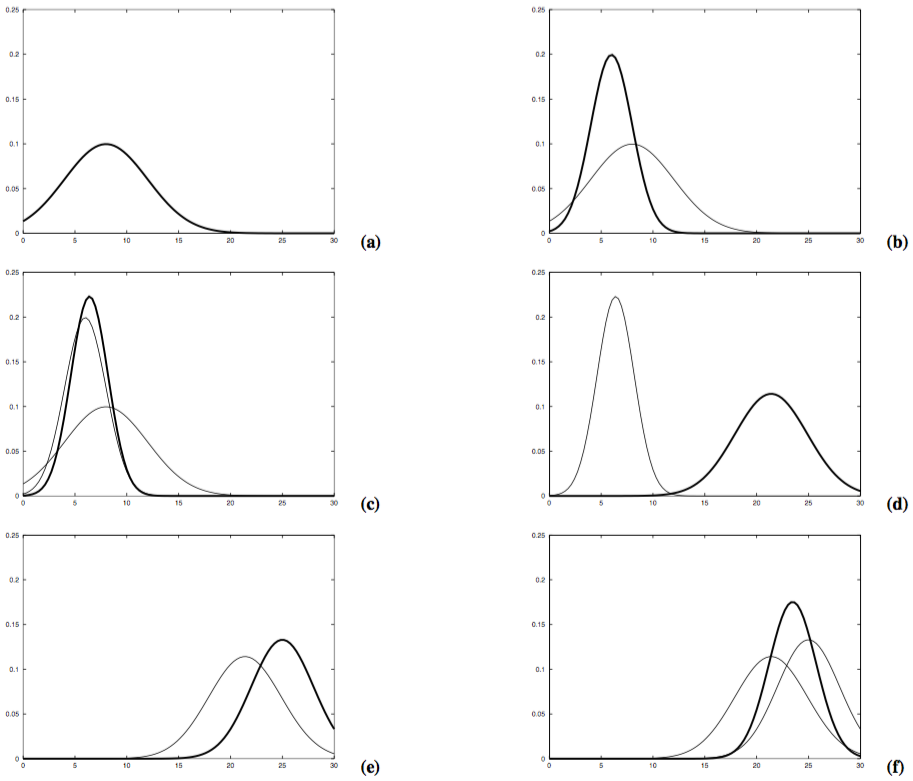
\includegraphics[scale=0.45]{images/KalmanFilterExample}
\caption{Kalman Filter example in a one-dimensional localization scenario}
\label{fig:kf_ex}
\end{figure}

\subsection{Extended Kalman filters}

The plain KF assumes that the system is linear in the state transitions and measurements with added Gaussian noise. This is however not the case in many systems and therefore the KF is inapplicable in many non-trivial problems.\\

To overcome this limitation of the plain KF, the extended Kalman Filter (EKF) can be used instead. In the EKF linearization is used to generate an approximation to the nonlinear system. This approximation to the true belief is represented by a mean value $\mu_t$ and a variance $\sigma_t^2$. Therefore the EKF represents its belief as the plain KF, but it uses an approximation instead of the exact belief.\\

The formal definition of the EKF is given in Algorithm \ref{alg:ekf_def1}.

\begin{center}
\begin{minipage}{.65\linewidth}
\alglanguage{pseudocode}
\begin{algorithm}[H]
\caption{Extended Kalman Filter}
\label{alg:ekf_def1}
\begin{algorithmic}[1]
\Procedure{ExtendedKalmanFilter}{$\mu_{t-1},\Sigma_{t-1},u_{t},z_{t}$}
  \State $\bar\mu_{t} = g(u_t,\mu_{t-1})$
  \State $\bar\Sigma_{t} = G_{t}\Sigma_{t-1}G_{t}^T + R_{t}$
  \State $K_{t} = \bar\Sigma_{t}H_{t}^T(H_{t}\bar{\Sigma}_{t}H_{t}^T+Q_{t})^{-1}$
  \State $\mu_{t} = \bar\mu_{t} + K_{t}(z_{t} - h(\bar{\mu_t}))$
  \State $\Sigma_{t} = (I - K_{t}H_{t})\bar\Sigma_{t}$
  \State \textbf{return} $\mu_{t}, \Sigma_{t}$
\EndProcedure
\end{algorithmic}
\end{algorithm}
\end{minipage}
\end{center}

The EKF in Algorithm \ref{alg:ekf_def1} looks very similar to the plain KF in Algorithm \ref{alg:kf_def1}. But the important difference are seen in line 2 and line 5, where the linear prediction of the KF are replaced by the linearized functions $g(u_t,\mu_{t-1})$ and $h(\bar{\mu_t})$, respectively. Also, the linear system matrices $A_t$ and $B_t$ have been replaced with the Jacobian $G_t$, and $C_t$ with $H_t$. The Jacobians are a consequence of the linearized operation.

%!TEX root = ..\Master.tex

\section{Particle Filters}
%!TEX root = ../Master.tex

\section{Path Planning} % (fold)
\label{sec:path_planning}

When a robot has located itself the next task might be to go somewhere. The task of planning a path from the location of the robot to some goal location is, when talking about robots, often referred to as robot motion planning. The problem to solve is to find the best possible path for the goal location when knowing the start location, the map and maybe some kind of cost function. This cost function can be thought of as the time it takes to follow a certain route. When introducing this cost function the best possible path is the minimum cost path. \\

\subsection{A* Algorithm} % (fold)
\label{sub:a_algorithm}

The path planning can be looked at as a search problem. A search problem is a problem with a set of nodes, an initial node and a goal node. The search problem can be solved by using a search algorithm. The search algorithm starts at the initial node and searches throughout the nodes in order to find the goal node. A variant of this search algorithm has been developed in order to handle the problem of path planning better. This algorithm is referred to as A* (pronounced A star). The steps of the algorithm is explained in the following section. \\

To understand the approach of the A* algorithm a couple of variables must be introduced.

\begin{itemize}
	\item The \emph{g} value is the cost of the path used to get to that node.

	\item The \emph{h} value is the number of nodes to pass to get to the goal node without taking obstacles into account. This can also be looked at as the displacement along both the x-axis and the y-axis of a node compared to the goal node.

	\item The \emph{f} value is the sum of the \emph{g} value and the \emph{h} value.\\
\end{itemize}

The algorithm also introduces three different lists.

\begin{itemize}
	\item The \emph{open} list is a list of nodes to be investigated. The list is sorted so that the node with the smallest \emph{f} value is the next node to be investigated. Nodes are being added to the \emph{open} list when a neighbor node is being investigated.

	\item The \emph{closed} list is a list of all nodes which have been investigated. This is used to keep track of these nodes in order to avoid investigation of a node twice or more.

	\item The \emph{action} list is a list which keeps track of which node was the previous node for all investigated nodes.\\
\end{itemize}

The procedure of the algorithm is as following. 

\begin{enumerate}
  \item The initial node is added to the \emph{open} list.

  \item The node in the \emph{open} list with the lowest \emph{f} value is chosen to be investigated. The chosen node is deleted from the \emph{open} list and added to the \emph{closed} list. 

  \item All neighbor nodes which are not in the \emph{closed} list are added to the \emph{open} list. All nodes are added to the \emph{action} list together with the information of which node was the previous node.
\end{enumerate}

Step two and three are repeated until the node from the \emph{open} list is the goal node. Then the planned path can be found. This is done by introducing a new list called \emph{path}. The goal node is added to this list and from the \emph{action} list the previous node is known. This node is added to the \emph{path} list. The previous node to this node is looked up in the \emph{action} list and so on until the previous node is the initial node. After reversing the \emph{path} list the path for the robot is planned. \\

% subsection a_algorithm (end)

\subsection{Path Smoothing} % (fold)
\label{sub:path_smoothing}

As described the A* algorithm results in a \emph{path} list. This planned path might be a very cornered path with lots of sharp turns for the robot to do. If this is not desirable for the robot the path can be smoothed. \\

For the smoothing algorithm all nodes in the \emph{path} list are denoted $x_i$ where $i$ is the number the node has in the list. All nodes in the \emph{smoothened path} list is denoted $y_i$. The algorithm has to solve a minimization problem. The \emph{smoothened path} list is initialized to be the same as the \emph{path} list as it is denoted in \autoref{eq:init_smooth_path}.

\begin{equation}
\label{eq:init_smooth_path}
y_i = x_i
\end{equation}

The minimization problem is defined in \autoref{eq:minimize}. The factor $\alpha$ sets how smooth the path is going to be. The larger value of $\alpha$, the more smooth the path gets. 

\begin{equation}
\label{eq:minimize}
\text{minimize\ } (x_i - y_i)^2 - \alpha (y_i - y_{i+1})^2
\end{equation}

In an implementation of the path smoothening algorithm two values are used to regulate for the smoothening, $\alpha$ and $\beta$. The $\alpha$ value yields how much the path should smoothen and the $\beta$ value yields how much the path should look like the original path. The path is being changed until the new change is smaller than some tolerance. An example of an implementation is shown in \autoref{smooth_path}. Notice that when the algorithm is implemented the initial node and the goal node has to stay unchanged.

\begin{lstlisting}[caption=Implementation example of path smoothing., label=smooth_path, language=Matlab]
function newpath = smoothPath(path, alpha, beta, tolerance)
    [length, width] = size(path);
    newpath = zeros(length,width);
    
    for i = 1:length
        for j = 1:width
            newpath(i,j) = path(i,j);
        end
    end
    
    change = tolerance;
    while change >= tolerance
        change = 0;
        for n = 2:length - 1
            for m = 1:width
                aux = newpath(n,m);
                newpath(n,m) = newpath(n,m) + alpha * (path(n,m) - newpath(n,m));
                newpath(n,m) = newpath(n,m) + beta * (newpath(n-1,m)+newpath(n+1,m)-2*newpath(n,m));
                change = change + abs(aux - newpath(n,m));
            end
        end
    end
end
\end{lstlisting}

% subsection path_smoothing (end)
% section path_planning (end)
%!TEX root = ..\Master.tex

\section{PID Control}
%!TEX root = ../Master.tex

\section{SLAM}

A fundamental problem involved with AI in robotics is localization and mapping. This problem arises when the robot does not have a map of the environment and do not know it's pose. Usually the only information the robot have at it's disposal are measurements and control-inputs. This problem is commonly referred to as \textit{Simultaneous Localization And Mapping} abbreviated or \textit{SLAM}.\\

A technique to solve the SLAM problem is called GraphSLAM. As the name suggest, this technique represents the robots poses and landmarks as nodes in a graph and constraints between poses, resulting from measurements, are encoded on the edges between nodes. An edge between two nodes therefore represents a spatial constraint relating the two robot poses. Since constraints are generated from measurements which we represent as Gaussians because of measurement uncertainty, the goal then, is to find a configuration of the nodes that minimize the error introduced by the constraints.\\

We represent the constraints between poses and landmarks using a matrix $\Omega$ and a vector $\xi$. The matrix describes which object (poses and landmarks) in the environment that are related, and the vector contains a value for this relationship which could be a distance between the objects. When new constraint are generated by the robot, the matrix and vector is modified by adding the constraints to a subset of the matrix and vector.\\

Once the constraints have been defined in the matrix and vector pair, the best estimate of the robot poses and landmarks positions can be calculated by inverting the matrix $\Omega$ and multiplying it with the vector $\xi$ as shown by Equation \ref{eq:slam_est}.

\begin{equation}
\label{eq:slam_est}
\mu = \Omega^{-1}\xi
\end{equation}

To summarize, in the graph-based SLAM technique, we add information to the matrix $\Omega$ and vector $\xi$ every time an constraint is encountered, and when we are done gathering constraints a simple procedure is run which gives the robot poses and landmark locations.

\subsection{GraphSLAM example}

In this section a simple example is given on how to use GraphSLAM which involves defining constraints and solving a system of equations to obtain robot and landmark locations.\\

Given the graph in \autoref{fig:slam_ex} which shows three robot poses and a landmark, we need a matrix of size $4\times4$ and a vector of size 4 to describe all the constraints. The initial position of the robots is $x_0 = -3$ and we can define the local constraints of movement $x_0 \rightarrow x_1$ and $x_1 \rightarrow x_2$ as Equation \ref{eq:slam_pose_rel1_a} and \ref{eq:slam_pose_rel1_b}, respectively.

\begin{equation}
\label{eq:slam_pose_rel1_a}
x_1 = x_0 + 5
\end{equation}

\begin{equation}
\label{eq:slam_pose_rel1_b}
x_2 = x_1 + 3
\end{equation}

Which gives constraints in Equation \ref{eq:slam_pose_rel2_a} - \ref{eq:slam_pose_rel3_b}.

\begin{equation}
\label{eq:slam_pose_rel2_a}
x_0 - x_1 = -5
\end{equation}

\begin{equation}
\label{eq:slam_pose_rel2_b}
x_1 - x_0 = 5
\end{equation}

\begin{equation}
\label{eq:slam_pose_rel3_a}
x_1 - x_2 = -3
\end{equation}

\begin{equation}
\label{eq:slam_pose_rel3_b}
x_2 - x_1 = 3
\end{equation}

Adding constraints in Equation \ref{eq:slam_pose_rel2_a} and \ref{eq:slam_pose_rel2_b} together with the initial position of the robot, gives the matrix and vector shown in Equation \ref{eq:slam_matrix1}.

\begin{equation}
\label{eq:slam_matrix1}
\begin{bmatrix}
2 & -1 & 0 & 0 \\
-1 & 1 & 0 & 0 \\
0 & 0 & 0 & 0 \\
0 & 0 & 0 & 0 \\
\end{bmatrix}
\begin{bmatrix}
-8 \\
5 \\
0 \\
0 \\
\end{bmatrix}
\end{equation}

Adding the constraint relating $x_1$ to $x_2$ results in the matrix and vector shown in Equation \ref{eq:slam_matrix2}.

\begin{equation}
\label{eq:slam_matrix2}
\begin{bmatrix}
2 & -1 & 0 & 0 \\
-1 & 2 & -1 & 0 \\
0 & -1 & 1 & 0 \\
0 & 0 & 0 & 0 \\
\end{bmatrix}
\begin{bmatrix}
-8 \\
2 \\
3 \\
0 \\
\end{bmatrix}
\end{equation}

Now the constraints relating the robot poses is added to the landmark.

\begin{figure}[H]
\centering
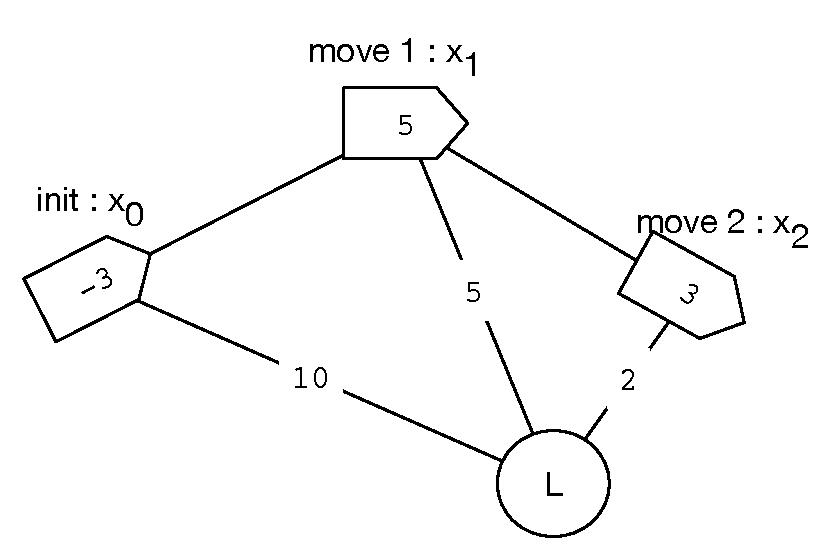
\includegraphics[scale=0.70]{images/ex_slam_graph}
\caption{GraphSLAM example}
\label{fig:slam_ex}
\end{figure}

The relation between the three poses and the landmark is giving by Equation \ref{eq:slam_lan_rel1} - \ref{eq:slam_lan_rel3}.

\begin{equation}
\label{eq:slam_lan_rel1}
L = x_0 + 10
\end{equation}

\begin{equation}
\label{eq:slam_lan_rel2}
L = x_1 + 5
\end{equation}

\begin{equation}
\label{eq:slam_lan_rel3}
L = x_2 + 2
\end{equation}

Which gives the constraints for $x_0 \rightarrow L$.

\begin{equation}
\label{eq:slam_lan_cons1_a}
x_0 - L = -10
\end{equation}

\begin{equation}
\label{eq:slam_lan_cons1_b}
L - x_0 = 10
\end{equation}

And for $x_1 \rightarrow L$.

\begin{equation}
\label{eq:slam_lan_cons2_a}
x_1 - L = -5
\end{equation}

\begin{equation}
\label{eq:slam_lan_cons2_b}
L - x_1 = 5
\end{equation}

And lastly for $x_2 \rightarrow L$.

\begin{equation}
\label{eq:slam_lan_cons3_a}
x_2 - L = -2
\end{equation}

\begin{equation}
\label{eq:slam_lan_cons3_b}
L - x_2 = 2
\end{equation}

Adding these constraints to the matrix and vector in Equation \ref{eq:slam_matrix2} produces the matrix and vector in Equation \ref{eq:slam_matrix3}.

\begin{equation}
\Omega =
\label{eq:slam_matrix3}
\begin{bmatrix}
3 & -1 & 0 & -1 \\
-1 & 3 & -1 & -1 \\
0 & -1 & 2 & -1 \\
-1 & -1 & -1 & 3 \\
\end{bmatrix}\,
\xi =
\begin{bmatrix}
-18 \\
-3 \\
1 \\
17 \\
\end{bmatrix}
\end{equation}

Solving this system using Equation \ref{eq:slam_est} produces the best estimate $\mu$ shown in Equation \ref{eq:slam_calc}.

\begin{equation}
\label{eq:slam_calc}
\mu = \Omega^{-1}\xi = 
\begin{bmatrix}[2.2]
1 & 1 & 1 & 1 \\
1 & \dfrac{13}{8} & \dfrac{3}{2} & \dfrac{11}{8} \\
1 & \dfrac{3}{2} & 2 & \dfrac{3}{2} \\
1 & \dfrac{11}{8} & \dfrac{3}{2} & \dfrac{13}{8} \\
\end{bmatrix}
\begin{bmatrix}[2.2]
-18 \\
-3 \\
1 \\
17 \\
\end{bmatrix} =
\begin{bmatrix}[2.2]
-3 \\
2 \\
5 \\
7 \\
\end{bmatrix}
\end{equation}

Meaning that the positions of the robot and the landmark are $x_0 = -3$, $x_1 = 2$, $x_2 = 5$, and $L = 7$. Note that in Equation \ref{eq:slam_matrix3} matrix $\Omega$ has zeros in positions $\Omega_{3,1}$ and $\Omega_{1,3}$ meaning that there is no constraint between $x_0$ and $x_2$. This can also be seen in \autoref{fig:slam_ex} by the absence of an edge between these two nodes.


\chapter{Project}

%----------------------------------------------------------------------------------------
%	REFERENCE LIST
%----------------------------------------------------------------------------------------
\bibliography{bibtex/references}
\fxnote{Remove "Pattern recognition and machine learning" from references.}

%----------------------------------------------------------------------------------------

\end{document}